%# -*- coding: utf-8-unix -*-
% !TEX program = xelatex
% !TEX root = ../thesis.tex
% !TEX encoding = UTF-8 Unicode
%%==================================================
%% chapter02.tex for SJTU Master Thesis
%% based on CASthesis
%% modified by wei.jianwen@gmail.com
%% Encoding: UTF-8
%%==================================================

\chapter{Finding key nodes on two layer networks}
\label{chap:finding key nodes on two layer networks}
In this chapter, it would be investigated that what nodes are important to keep or change their orientation on two-layer networks. There exist many methods to find key nodes, such as pagerank, degree centrality, and eigenvector centrality. And, in \parencite{mesgari2015, huang2014}, it has been proved that multiple indicators are useful to identify key nodes and prevent the slow way to find important nodes. Based on these methods such as single node centrality and combined node centrality, it would be researched that which method is the most effective and the most influential for changing state on two layers.  

\section{Method for finding key nodes}
\label{sec:method for finding key nodes}
As initial condition for finding key nodes, each layer is made of \textit{BA} network with $2048$ nodes, $K=3$, and $1$ external edge. Each simulation takes $100$ steps, and $100$ simulations are considered for average results. To demonstrate the difference of network state clearly, for finding key nodes on layer A, the parameters would be set to be negative consensus state. Then, as the stubborn nodes on layer A are increased, the network state would be gradually changed into positive state.  Inversely for finding key nodes on layer B, the parameters would be set to be positive consensus state. Then, as the stubborn nodes on layer B are increased, the network state would be gradually changed into negative state.
Here is the way to find key nodes by using single node centrality..
\begin{enumerate}
	\item All nodes are ranked by 6 node centralities(pagerank, degree, eigenvector, closeness, betweenness).
	\item The nodes would be deactivated from high ranked order until the state of network has significant difference, i.e. the ratio of stubborn node would be increased according to high ranked order. 
	\item The results would be compared according to node centralities. If the least ratio of stubborn node makes the largest difference of network state, its node centrality is the most influential for competition of the interconnected network
\end{enumerate}

And, we would research the way to recognize important node by using multiple indicator such as combined node centrality. Combined node centrality is made up with several selected node centralities. When it is proven that a node centrality is effective to find key nodes through the simulations, it would be selected as a factor of combined node centrality. $2$ or $3$ node centralities would be selected. 
The way to recognize key nodes by using combined node centrality follow like this steps. 
\begin{enumerate}
	\item All nodes are ranked by each selected node centralities. All nodes has the ranks as the number of selected node centralities.  
	\item Combined node centrality is the summation of all ranks which a node has. 
	\item All nodes are ranked again by combined node centrality. As the combined node centrality is smaller, a node are ranked higher.        
	\item The nodes would be deactivated from high ranked order until the state of network has significant difference, i.e. the ratio of stubborn node would be increased according to high ranked order. 
\end{enumerate}
 
\section{Key nodes on layer A}
\begin{figure}[!htb]
	\centering
	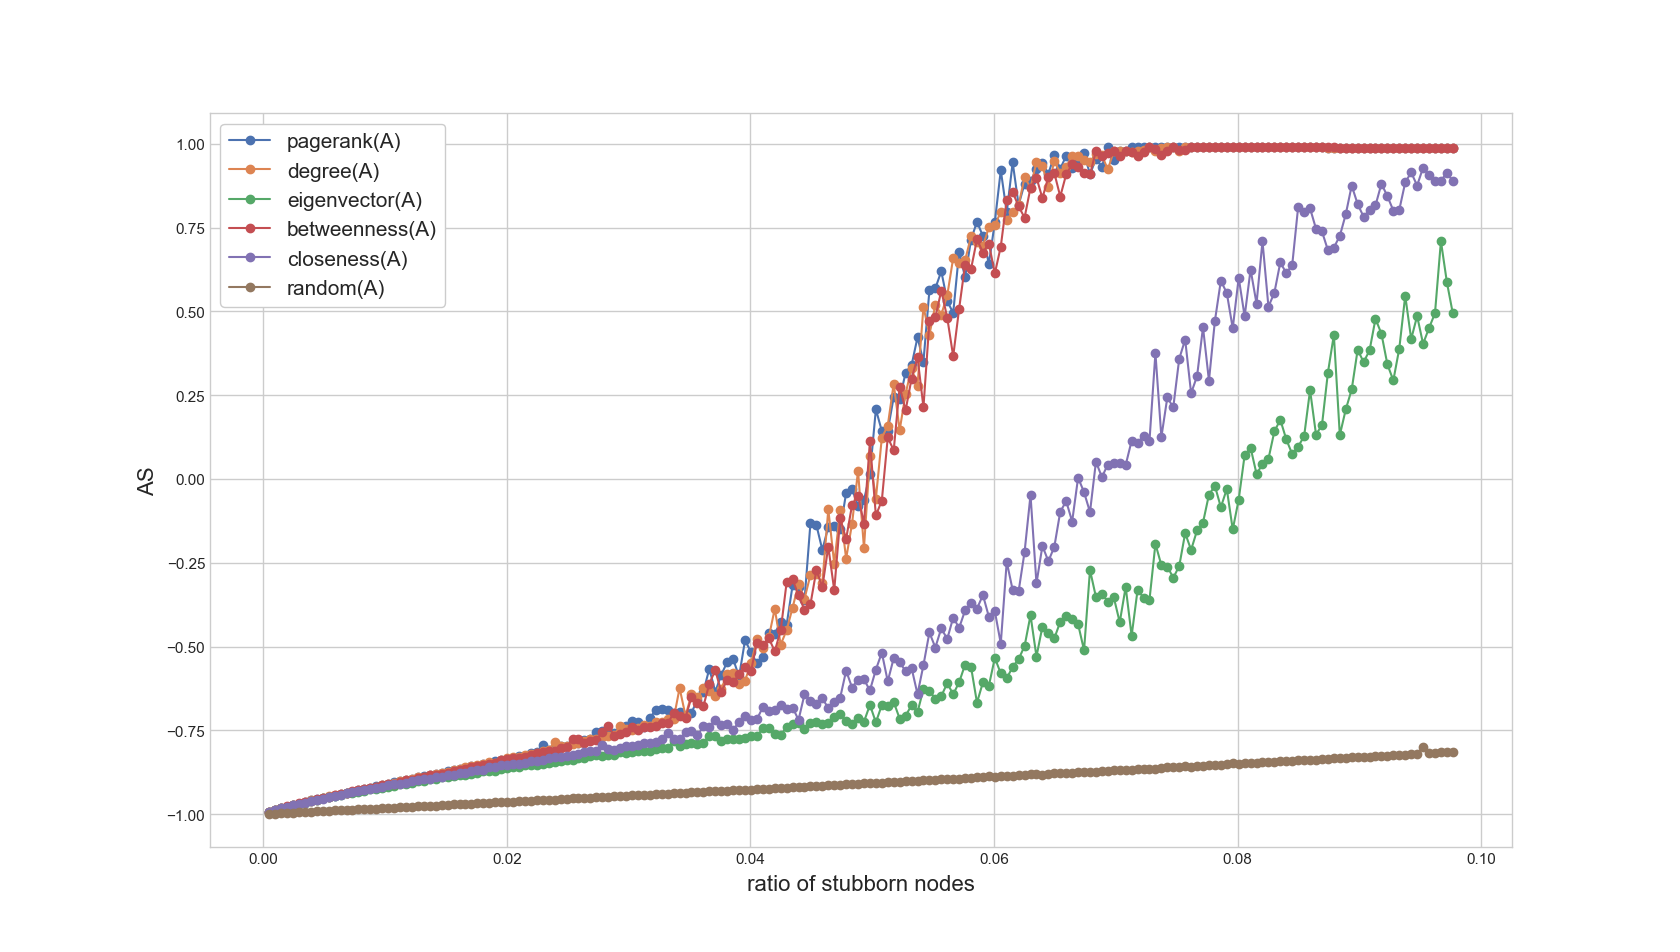
\includegraphics[width=\hsize]{figure/chap5_keynode_A_1.png}
	\caption{Simulation results according to single node centrality for finding key nodes on layer A}
	\label{chap5_keynode_A_1}
\end{figure}
To find key nodes on layer A, parameters are set to be negative consensus state like $p=0.2, v=0.4$. Firstly, Only node centralities would be compared as single indicator for identifying key nodes. 5 node centralities(pagerank, degree, eigenvector, closeness, betweenness) are used as a single indicator. And random selected nodes are compared with 5 node centralities. 
Fig.~\ref{chap5_keynode_A_1} shows the simulation result for single node centralities. As shown in Fig.~\ref{chap5_keynode_A_1}, the rank of effective way to recognize important nodes follow like this. 
\begin{enumerate}
	\item pagerank > degree > betweenness  
	\item closeness
	\item eigenvector       
	\item random
\end{enumerate}
Pagerank, degree centrality and betweenness centrality have almost same results. But, pagerank reaches positive consensus firstly, and then degree centrality reaches secondly though the gap between them is very slight. The next rank order is like closeness, eigenvector and random. To clarify which method is the best and most effective, we would use the indexes \textit{ `stability'} and \textit{`distance' } for measuring stability and distance to end state. \textit{`stability'} and \textit{`distance'} are derived as following steps. 
\begin{enumerate}
	\item As described in \ref{sec:method for finding key nodes}, all \textit{AS}s are calculated according to ratio of stubborn nodes   
	\item all \textit{AS}s are arranged according to ratio of stubborn nodes. 
	\item \textit{`stability'} is defined as the absolute value of gap between a \textit{AS} and the next \text{AS}. Fluctuation of stability shows which method is the best and fastest way to find key nodes. Small fluctuation is the best and stablest way to identify key nodes. 
	\item \textit{`distance'} is the summation of all \textit{`stability'}. As the \textit{distance} is large, the method is slow and unstable to recognize key nodes.
\end{enumerate}
\begin{figure}[!htb]
	\centering
	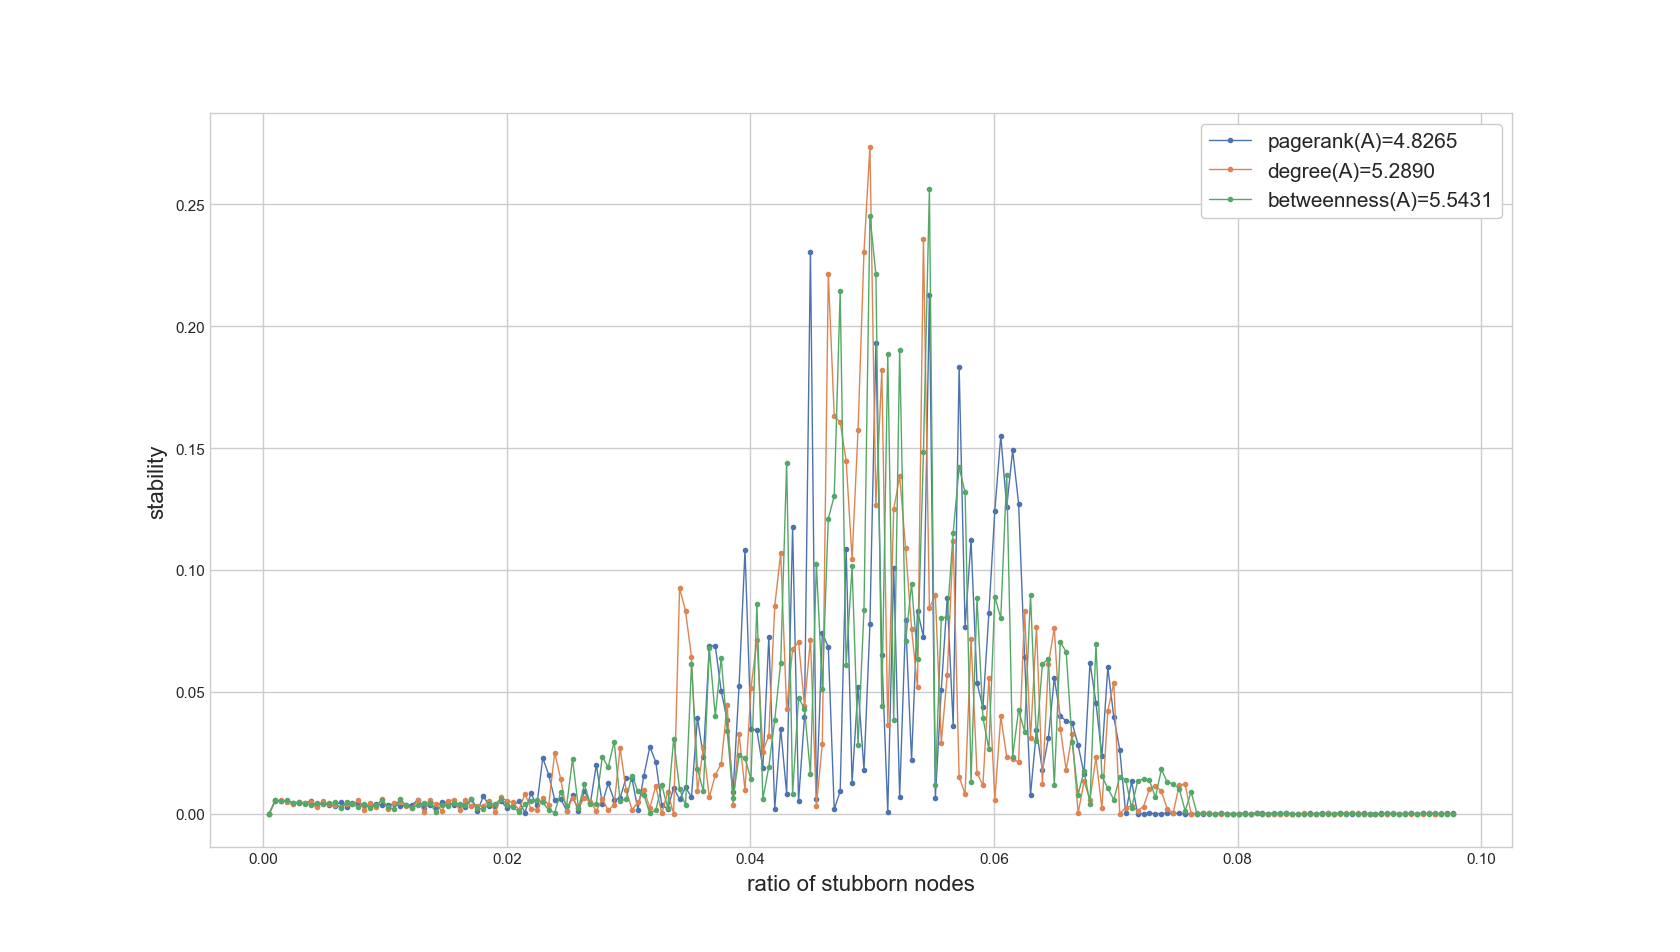
\includegraphics[width=\hsize]{figure/chap5_keynode_A_2.png}
	\caption{Comparison of single indicators according to stability and distance  }
	\label{chap5_keynode_A_2}
\end{figure}

Fig.~\ref{chap5_keynode_A_2} shows the simulation results by using indexes, \textit{distance} and \textit{stability}. The order is distance is like pagerank(4.8265), degree(5.2890), and betweenness(5.5431). Stability of fluctuation is also shown as same order. Pagerank has the smallest fluctuation and distance. Therefore, it could be thought that pagerank is the best and most efficient method to recognize key nodes as a single indicator.  
Next, we would try to find key node by using multiple indicators. It could be known that pagerank, degree and betweenness are effective to identify key nodes. Therefore, we would select these node centralities as the factors of combined node centrality.
Fig.~\ref{chap5_keynode_A_3} presents the result of combined node centrality with pagerank and degree. 
\begin{figure}[!htb]
	\centering
	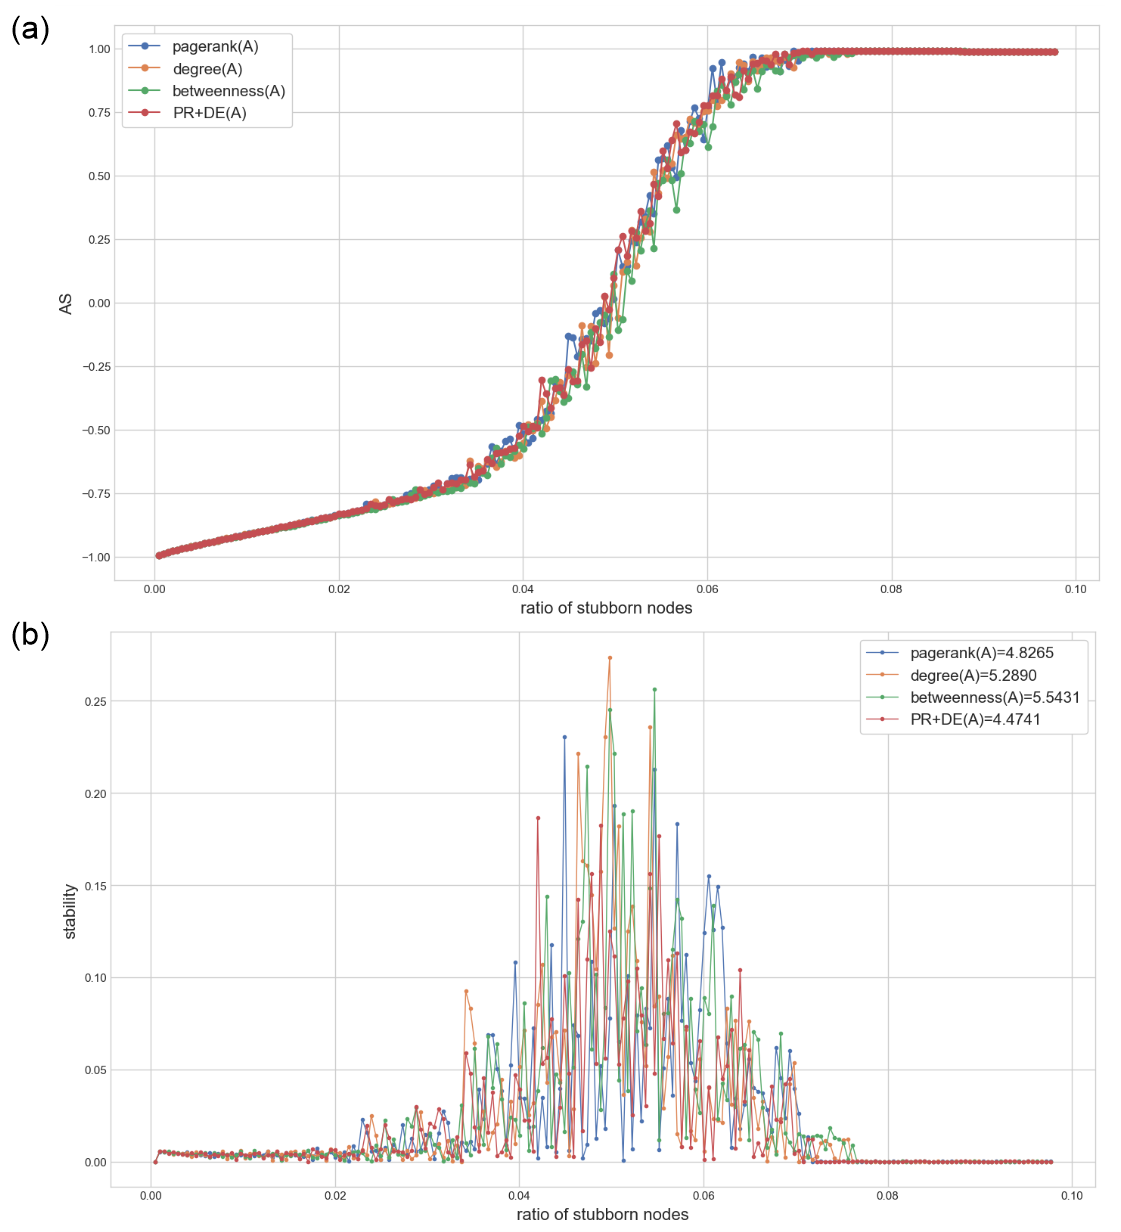
\includegraphics[width=\hsize]{figure/chap5_keynode_A_3.png}
	\caption{Comparison between multiple indicator(pagerank and degree) and single indicator:
	(a) AS with increasing the ratio of stubborn nodes, (b) Stability with increasing the ratio of stubborn nodes}
	\label{chap5_keynode_A_3}
\end{figure}
In Fig.~\ref{chap5_keynode_A_3} (a), combined node centrality has almost same result with single node centrality(pagerank, degree, betweenness). However, Fig.~\ref{chap5_keynode_A_3} (b) presents that the multiple indicator(PR+DE) has the smallest distance and fluctuation. It could be found out that multiple indicator is more effective than single indicator.  




  
  
  
\section{Key nodes on layer B}
To find key nodes on layer B, parameters are set to be positive consensus state like $p=0.3, v=0.5$. Firstly, Only node centralities would be compared as single indicator for identifying key nodes. 5 node centralities(pagerank, degree, eigenvector, closeness, betweenness) are used as a single indicator. And random selected nodes are compared with 5 node centralities. 
Fig.~\ref{chap5_keynode_A_1} shows the simulation result for single node centralities. As shown in Fig.~\ref{chap5_keynode_A_1}, the rank of effective way to recognize important nodes follow like this. 
\begin{enumerate}
	\item pagerank > degree > betweenness  
	\item closeness
	\item eigenvector       
	\item random
\end{enumerate}
Pagerank, degree centrality and betweenness centrality have almost same results. But, pagerank reaches positive consensus firstly, and then degree centrality reaches secondly though the gap between them is very slight. The next rank order is like closeness, eigenvector and random. It could be known that pagerank, degree and betweenness are effective to identify key nodes. There, we would select 2 or 3 node centralities as the factors of combined node centrality. 





\section{Key nodes on two layers with different structures}
In this section, we use the hierarchical models described in chapter.~\ref{chap:competition on two layer with various structural network} with \textit{BA} network. Each layer consists of \textit{BA} network with $k=3$. Layer A has 2048 nodes, and layer B has $256$ nodes. We denote these models as \textit{HM(8) with BA(3)}. 



\section{Conclusion}
By using node centrality, key nodes on each layer have been found out. 
And under the hierarchical models, key nodes also have been found out. 